% REMEMBER: You must not plagiarise anything in your report. Be extremely careful.

\documentclass{l4proj}
\usepackage{subfiles}
\usepackage{pdfpages}

    
%
% put any additional packages here
%

\begin{document}

%==============================================================================
%% METADATA
\title{RViT - A Requirement and Value Identification Tool for Prioritisation}
\author{Niamh Gillespie}
\date{March 22, 2024}

\maketitle

%==============================================================================
%% ABSTRACT
\begin{abstract}
    Current agile project management tooling often comes with a considerable administrative and 
    
    Every abstract follows a similar pattern. Motivate; set aims; describe work; explain results.
    \vskip 0.5em
    ``XYZ is bad. This project investigated ABC to determine if it was better. 
    ABC used XXX and YYY to implement ZZZ. This is particularly interesting as XXX and YYY have
    never been used together. It was found that  
    ABC was 20\% better than XYZ, though it caused rabies in half of subjects.''
\end{abstract}

%==============================================================================

\chapter*{Acknowledgements}

I would like to thank my supervisor, Peggy Gregory, for her continued help and support throughout the duration of the project. I would also like to thank the developers who took part in my pilot study and user evaluation, their feedback was invaluable.

I would also like to thank my family and friends for putting up with me talking about RViT 24-7.

%==============================================================================
% EDUCATION REUSE CONSENT FORM
% If you consent to your project being shown to future students for educational purposes
% then insert your name and the date below to  sign the education use form that appears in the front of the document. 
% You must explicitly give consent if you wish to do so.
% If you sign, your project may be included in the Hall of Fame if it scores particularly highly.
%
% Please note that you are under no obligation to sign 
% this declaration, but doing so would help future students.
%
\def\consentname {Niamh Gillespie} % your full name
\def\consentdate {22 March 2024} % the date you agree
%
\educationalconsent


%==============================================================================
\tableofcontents

%==============================================================================
%% Notes on formatting
%==============================================================================
% The first page, abstract and table of contents are numbered using Roman numerals and are not
% included in the page count. 
%
% From now on pages are numbered
% using Arabic numerals. Therefore, immediately after the first call to \chapter we need the call
% \pagenumbering{arabic} and this should be called once only in the document. 
%
% Do not alter the bibliography style.
%
% The first Chapter should then be on page 1. You are allowed 40 pages for a 40 credit project and 30 pages for a 
% 20 credit report. This includes everything numbered in Arabic numerals (excluding front matter) up
% to but excluding the appendices and bibliography.
%
% You must not alter text size (it is currently 10pt) or alter margins or spacing.
%
%
%==================================================================================================================================
%
% IMPORTANT
% The chapter headings here are **suggestions**. You don't have to follow this model if
% it doesn't fit your project. Every project should have an introduction and conclusion,
% however. 
%
%==================================================================================================================================
\chapter{Introduction}

% reset page numbering. Don't remove this!
\pagenumbering{arabic} 

\subfile{Introduction}


%==================================================================================================================================
\chapter{Background}
\subfile{Background}
%==================================================================================================================================
\chapter{Requirement Analysis}
\subfile{Requirements}

%==================================================================================================================================
\chapter{Design}
\subfile{Design}

%==================================================================================================================================
\chapter{Implementation}
\subfile{Implementation}

%==================================================================================================================================
\chapter{Evaluation} 
\subfile{Evaluation}
%==================================================================================================================================
\chapter{Conclusion}    
\subfile{Conclusion}

%==================================================================================================================================
%
% 
%==================================================================================================================================
%  APPENDICES  

\begin{appendices}

\chapter{Final Deliverable}

\chapter{Database Schema}

\chapter{Ethics Checklist}
\centerline{
\includegraphics[width=1.2\textwidth, page=1]{dissertation/appendices/2549880G_ethics_checklist.pdf}
}

\includepdf[width=1.2\textwidth, pages={2}]{appendices/2549880G_ethics_checklist.pdf}



\chapter{User Evaluation Survey}
\begin{center}
\centering
\includegraphics[width=1\textwidth, page=1]{dissertation/appendices/FirstPageEvaluationSurvey.png}
\end{center}

\includepdf[pages={2-5}]{appendices/UserEvaluationSurveyForm.pdf}

\chapter{User evaluation survey responses}

\chapter{Qualitative Coding of Text Responses from User Evaluation}

\end{appendices}

%==================================================================================================================================
%   BIBLIOGRAPHY   

% The bibliography style is abbrvnat
% The bibliography always appears last, after the appendices.

\bibliographystyle{abbrvnat}

\bibliography{l4proj}

\end{document}
